% --------------------------------------------------------------
%  BEAMER TEMPLATE – 30min technical presentation
% --------------------------------------------------------------
\documentclass[12pt]{beamer}

% --------------------------------------------------------------
%  Theme & colour scheme
% --------------------------------------------------------------
\usetheme{Madrid}          % you may switch to Warsaw, Berlin, …
\usecolortheme{dolphin}    % or beaver, crane, …

% --------------------------------------------------------------
%  Packages
% --------------------------------------------------------------
\usepackage{fontspec}
\usepackage{graphicx}      % figures
\usepackage{booktabs}      % tables
\usepackage{hyperref}      % links
\usepackage{amsmath,amssymb}
\usepackage{listings}      % code listings
\usepackage{caption}

% --------------------------------------------------------------
%  Colors
% --------------------------------------------------------------
\definecolor{burntOrange}{HTML}{BF5700}
\definecolor{myGray}{HTML}{EEEEEE}
\definecolor{myBlack}{HTML}{111111}
\setbeamercolor{structure}{fg=burntOrange, bg=myBlack}
\setbeamercolor{title}{fg=myBlack, bg=burntOrange}
\setbeamercolor{frametitle}{bg=burntOrange,fg=myBlack }
\setbeamercolor{block title}{bg=burntOrange, fg=myBlack}
\setbeamercolor{block body}{bg=myGray, fg=myBlack}
\setbeamercolor{background canvas}{bg=myBlack!90}
\setbeamercolor{normal text}{fg=myGray}
\setbeamercolor{section in toc}{fg=myGray, bg=myBlack}

\author[Karl Solomon]{\large Karl Solomon}

% --------------------------------------------------------------
%  BEGIN DOCUMENT
% --------------------------------------------------------------
\begin{document}

% --------------------------------------------------------------
%  Title / author / date
% --------------------------------------------------------------
\title[SYNK 4K: Wireless Video Platform]{\Huge SYNK 4K:\\Wireless Video}
\subtitle{Technical Overview}
\institute[Stryker Endoscopy]{\href{mailto:karl.solomon20@gmail.com}{karl.solomon20@gmail.com}}
\date{\today}


% --------------------------------------------------------------
%  Font
% --------------------------------------------------------------
\setmainfont{JetBrainsMono Nerd Font}[Contextuals=Alternate, Ligatures = TeX]
\setmonofont{JetBrainsMono Nerd Font}[Contextuals=Alternate, Ligatures = TeX]

% --------------------------------------------------------------
%  Background
% --------------------------------------------------------------
\setbeamertemplate{navigation symbols}{}
% \setbeamertemplate{
%     \color{myGray!5}\rule{\paperwidth}{\paperheight}
% }

% --------------------------------------------------------------
%  Bullets
% --------------------------------------------------------------
\setbeamertemplate{itemize items}[circle]
\setbeamertemplate{enumerate items}[square]

% --------------------------------------------------------------
%  Title page
% --------------------------------------------------------------
\begin{frame}
    \titlepage
\end{frame}

% --------------------------------------------------------------
%  Outline (Table of contents)
% --------------------------------------------------------------
\begin{frame}{Outline}
    \tableofcontents
\end{frame}

% ==============================================================
%  SECTION 0 – About Me
% ==============================================================

\section{About Me}

\begin{frame}{About Me - Interests}
    \begin{figure}[ht]
        \centering
        
\includegraphics[width=0.3\textwidth]{~/science/resources/espresso.png}
        
\includegraphics[width=0.25\textwidth]{~/science/resources/radar.png}
        
\includegraphics[width=0.2\textwidth]{~/science/resources/bbq.jpg}
        
\includegraphics[width=0.4\textwidth]{~/science/resources/surface.jpeg}
        
\includegraphics[width=0.30\textwidth]{~/science/resources/soccer.jpg}
    \end{figure}
\end{frame}

\begin{frame}{About Me - Projects}
    \begin{figure}[ht]
        \centering
        
\includegraphics[width=0.25\textwidth]{~/science/resources/DeepBrain.jpg}
        
\includegraphics[width=0.35\textwidth]{~/science/resources/1688.png}
        
\includegraphics[width=0.3\textwidth]{~/science/resources/synk4k.png}
        
\includegraphics[width=0.3\textwidth]{~/science/resources/4090.png}
        
\includegraphics[width=0.15\textwidth]{~/science/resources/orin.png}
        
\includegraphics[width=0.4\textwidth]{~/science/resources/hopper1.jpg}
    \end{figure}
\end{frame}


% ==============================================================
%  SECTION 1 – Overview 
% ==============================================================

\section{Overview}

\begin{frame}{SYNK 4K – Overview}
    \begin{itemize}
        \item Surgical application
        \item Ultra low latency 4K60 video
        \item Incredibly stable \& high QoS link
        \item Coexist in 5GHz (incl. DFS in TDWR)
        \item Multicast
    \end{itemize}
    \begin{figure}[ht]
        \centering
        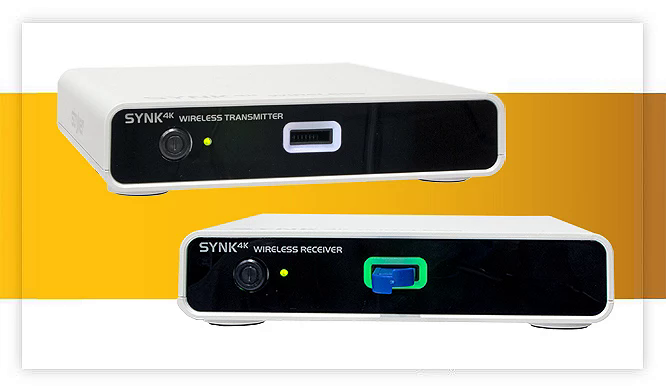
\includegraphics[width=0.6\textwidth]{./resources/synk4k.png}
    \end{figure}
\end{frame}

\begin{frame}{SYNK 4K – Overview}
    \begin{figure}[ht]
        \centering
        
\includegraphics[width=0.8\textwidth]{~/science/resources/stack.png}
        \caption{Software Stack}
    \end{figure}
\end{frame}

% ==============================================================
%  SECTION – Project Lifecycle
% ==============================================================
\section{Project Lifecycle}
\begin{frame}{SYNK 4K - Product Lifecycle}
    \begin{figure}[ht]
        \centering
        
\includegraphics[width=0.4\textwidth]{~/science/resources/components.jpg}
        
\includegraphics[width=0.4\textwidth]{~/science/resources/p2.png}
        
\includegraphics[width=0.4\textwidth]{~/science/resources/prototype.jpg}
        
\includegraphics[width=0.4\textwidth]{~/science/resources/p3.jpg}
    \end{figure}
\end{frame}

\begin{frame}{SYNK 4K - Test Lifecycle}
    \begin{figure}[ht]
        \centering
        
\includegraphics[width=0.3\textwidth]{~/science/resources/stressTest.jpg}
        
\includegraphics[width=0.3\textwidth]{~/science/resources/testFixture.jpg}
        
\includegraphics[width=0.3\textwidth]{~/science/resources/hospital.jpg}
    \end{figure}
\end{frame}

\begin{frame}{Team}
    \begin{figure}[ht]
        \centering
        
\includegraphics[width=0.4\textwidth]{~/science/resources/party.jpg}
        
\includegraphics[width=0.4\textwidth]{~/science/resources/sykTeam.jpg}
        
\includegraphics[width=0.4\textwidth]{~/science/resources/vendorTeam.jpg}
    \end{figure}
\end{frame}


% ==============================================================
%  SECTION – My Role & Architectural Leadership
% ==============================================================

\section{My Role}

\begin{frame}{My Role - Lead Software Engineer}
    \begin{itemize}
        \item Discovery \& vendor selection
        \item Component selection
        \item Board bringup
        \item Owner \& majority contributor of Arm Cortex-M software stack.
        \item Primary POC between R\&D teams.
        \item Authored all 62304 documents
    \end{itemize}
\end{frame}

\begin{frame}{My Role - A Typical Day}
    \begin{itemize}
        \item \textbf{Morning:} 50\% meetings, 50\% push through PRs
        \item \textbf{Afternoon:} Verify bugs resolved, help team move forward
        \item \textbf{Evening:} Code \& open PR
    \end{itemize}
\end{frame}

% ==============================================================
%  SECTION 4 – Metrics & Impact
% ==============================================================

\section{Metrics \& Recognition}
   \begin{frame}{Metrics \& Recognition}
       \begin{itemize}
           \item 150+ Pull requests merged
           \item 100+ JIRA bugs resolved
           \item 99+\% unit test code coverage
           \item 3 Customer complaints filed in 3 years
           \item 2x Employee of the month: Project
           \item "One Team": Division
           \item "Best Performance in a Leading Role": Division
       \end{itemize}
    \end{frame}

% ==============================================================
%  SECTION 
% ==============================================================
\section{Example Issue}

\begin{frame}{Flicker: Setup}
    \begin{itemize}
        \item Performing HDMI tuning requires renting lab space and takes 15-60 minutes per run.
        \item Takes 20-60 minutes per channel pending test settings
        \item 8K combinations
        \item Factory-defaults don't always work
        \item Other products' settings don't always work
        \item Seems to be very device \& setup specific
    \end{itemize}
\end{frame}

\begin{frame}{Flicker: Bayesian Approach}
    \begin{enumerate}
        \item Assume normal distribution about "optimal" parameter for all parameters
        \item Initial conditions: wide distribution about current settings
        \item Randomly sample each parameter relative to the current distribution
        \item Score is how "wide/open" is the eye
        \item Establish new distribution, toward progress, away from regression
        \item Repeat
    \end{enumerate}
\end{frame}

\begin{frame}{Flicker: Crowd Source Approach}
    \begin{figure}[ht]
    \centering
    
\includegraphics[width=0.5\textwidth]{~/science/resources/hdmiRedriver.jpg}
    \newline
    Rx\&Tx Eq, Gain, Output Swing, PreEmphasis, DeEmphasis, Tx Slew
\end{figure}
\end{frame}

% ==============================================================
%  SECTION 7 – Conclusion & Q&A
% ==============================================================

\section{Conclusion \& Q\&A}

\begin{frame}{Summary}
    \begin{itemize}
        \item All setups
        \item All devices
        \item All temperature conditions
        \item Resolved numerous undefined/open "flicker" bugs
        \item Key win that brought product from "good prototype" to "reliable for surgery"
    \end{itemize}
\end{frame}

\begin{frame}{Thank you!}
    \centering
    \large Questions?
    \vspace{1cm}
\end{frame}

\begin{frame}{Appendix: Two Generals}
    \begin{itemize}
\item \textbf{Situation}: Noisy environment causes QoS drop or DOS
\item \textbf{TX}: Scans environment, transmits video, receives QoS reports
\item \textbf{RX}: Scans environment, receives video, transmits QoS reports
\item \textbf{Problem1}: How to know when to jump channels \& to which channel
\item \textbf{Problem2}: QoS is bad, TX doesn't receive QoS packet
\item \textbf{Problem3}: RX turned off or interference is prohibitively high
\item \textbf{Problem4}: Reduce hops
\end{itemize}
\end{frame}



% --------------------------------------------------------------
%  END OF DOCUMENT
% --------------------------------------------------------------
\end{document}
